\documentclass[aps,prb,twocolumn,superscriptaddress,floatfix,longbibliography]{revtex4-2}

\usepackage[utf8]{inputenc}
\usepackage[spanish]{babel}
\usepackage{graphicx}
\usepackage{amsmath}
\usepackage{subcaption}
\usepackage{wrapfig} 
\usepackage[export]{adjustbox}

\usepackage{amsmath,amssymb} % math symbols
\usepackage{bm} % bold math font
\usepackage{graphicx} % for figures
\usepackage{comment} % allows block comments
\usepackage{textcomp} % This package is just to give the text quote '
%\usepackage{ulem} % allows strikeout text, e.g. \sout{text}

\usepackage[spanish]{babel}

\usepackage{enumitem}
\setlist{noitemsep,leftmargin=*,topsep=0pt,parsep=0pt}

\usepackage{xcolor} % \textcolor{red}{text} will be red for notes
\definecolor{lightgray}{gray}{0.6}
\definecolor{medgray}{gray}{0.4}

\usepackage{hyperref}
\hypersetup{
colorlinks=true,
urlcolor= blue,
citecolor=blue,
linkcolor= blue,
bookmarks=true,
bookmarksopen=false,
}

% Code to add paragraph numbers and titles
\newif\ifptitle
\newif\ifpnumber
\newcounter{para}
\newcommand\ptitle[1]{\par\refstepcounter{para}
{\ifpnumber{\noindent\textcolor{lightgray}{\textbf{\thepara}}\indent}\fi}
{\ifptitle{\textbf{[{#1}]}}\fi}}
%\ptitletrue  % comment this line to hide paragraph titles
%\pnumbertrue  % comment this line to hide paragraph numbers

% minimum font size for figures
\newcommand{\minfont}{6}

% Uncomment this line if you prefer your vectors to appear as bold letters.
% By default they will appear with arrows over them.
% \renewcommand{\vec}[1]{\bm{#1}}

%Cambiar Cuadros por Tablas y lista de...
%\renewcommand{\listtablename}{Índice de tablas}
\renewcommand{\tablename}{Tabla}
\renewcommand{\date}{Fecha}

\usepackage[bottom]{footmisc} %para que las notas al pie aparezcan en la misma página



\begin{comment}

%Comandos de interés:

* Para ordenar el documento:
\section{Introducción}
\section{\label{sec:Formatting}Formatting} %label para luego hacer referencia a esa sección

\ptitle{Start writing while you experiment} %pone nombre y título al documento dependiendo de si en el header están los comandos \ptitletrue y \pnumbertrue

* Ecuaciones:
\begin{equation}
a^2+b^2=c^2 \,.
\label{eqn:Pythagoras}
\end{equation}

* Conjunto de ecuaciones:
\begin{eqnarray}
\label{eqn:diagonal}
\nonumber d & = & \sqrt{a^2 + b^2 + c^2} \\
& = & \sqrt{3^2+4^2+12^2} = 13
\end{eqnarray}

* Para hacer items / enumerar:
\begin{enumerate}
  \item
\end{enumerate}

\begin{itemize}
  \item
\end{itemize}

* Figuras:
\begin{figure}[h]
    \includegraphics[clip=true,width=\columnwidth]{pixel-compare}
    \caption{}
     \label{fig:pixels}
\end{figure}

* Conjunto de figuras:
(no recuerdo)


* Para hacer referencias a fórmulas, tablas, secciones, ... dentro del documento:
\ref{tab:spacing}

* Para citar
Elementos de .bib
\cite{WhitesidesAdvMat2004}
url
\url{http://www.mendeley.com/}\\

* Agradecimientos:
\begin{acknowledgments}
We acknowledge advice from Jessie Zhang and Harry Pirie to produce Fig.\ \ref{fig:pixels}.
\end{acknowledgments}

* Apéndice:
\appendix
\section{\label{app:Mendeley}Mendeley}

* Bibliografía:
\bibliography{Hoffman-example-paper}

\end{comment}

\begin{comment}

Plots y tablas en orden:

* Figura de los cilindros con los PT100, la resistencia de referencia, la fuente, el multímetro y la computadora simbolizando el software de adquisisción de datos.
* Figura de los cilindros con la lampartira, la fuente que le da tensión y el multímetro para medir esa tensión

* Tabla de dimensiones de los cilindros
(la copio de prácticos anteriores)

* Figura del equipo de algto vacío (bomba mecánica, difusora, tubos, bridas, cámara, 3 cilindros...)
* Figura sobre cómo determinar epsilon (pirómetro, termocupla apoyados sobre cilindro exterior sin vacío)

PLOT PPAL:
* T vs t mostrando un gráfico lindo donde se vea bien el transitorio y el estacionario

SUBPLOTS:
* T vs t mostrando qué pasa si hay un cortocircuito interno que hace que la lámpara no prenda (se ven T bajas)
* T vs t mostrando qué pasa si no ponemos el telgopor
* T vs t mostrando qué pasa si falla el vacío
* T vs t mostrando qué pasa en el cilindro externo cuando agregamos N2
* T vs t mostrando qué pasa cuando cambiamos la potencia de la lamparita sobre la marcha



Determinación del producto de ctes
* T vs P recta para calcular la pendiente relacionada con el producto de constantes

Determinación de epsilon
* Gráfico Epsilon vs P

Bibliografía:
* Agregar referencia a la tabla de calibración R vs T
* Agregar referencia a que sacamos los datos de las áreas de un práctico de años anteriores

\end{comment}



\begin{document}

% Allows to rewrite the same title in the supplement
\newcommand{\mytitle}{Dinámica molecular en dos dimensiones}

\title{\mytitle}

\author{Pablo Chehade \\
    \small \textit{pablo.chehade@ib.edu.ar} \\
    \small \textit{Física computacional, Instituto Balseiro, CNEA-UNCuyo, Bariloche, Argentina} \\}



\maketitle

\section{Introducción}

\ptitle{Dinámica molecular a rasgos generales}

Describir la dinámica de un sistema de muchas partículas que interactúan con fuerzas conocidas no es sencillo. El problema se puede resolver exactamente para un sistema de dos cuerpos, pero para sistemas más grandes no hay una solución analítica y es necesario recurrir a métodos numéricos aproximados. De esta tarea se encarga justamente la dinámica molecular. Un algoritmo conocido para enfrentar este problema es el de Verlet, que calcula las posiciones $\mathbf{x}$ y velocidades $\mathbf{v}$ de la partícula $i$ a tiempo discretizado $n+1$ a partir de las expresiones
\begin{equation}
\begin{split}
\mathbf{x}^{n+1}_i = \mathbf{x}^n_i + h \mathbf{v}^n_i + \frac{h^2}{2}\mathbf{F}^n_i  \, \mathrm{y} \\
\mathbf{v}^{n+1}_i = \mathbf{v}^n_i + \frac{1}{2h}(\mathbf{F}^{n+1}_i + \mathbf{F}^n_i),
\end{split}
\label{eq:Verlet}
\end{equation}

donde el índice superior indica el tiempo al que está evaluada cada variable, $h$ es la unidad de tiempo discretizado y $F^n_i$ es la fuerza sobre la partícula $i$ debido a las interacciones con las demás partículas. En una primera aproximación dichas interacciones se pueden considerar clásicamente, de modo que $F^n_i$ estará dada por la ecuación de Newton:
\begin{equation}
F^n_i = \sum_{i \neq j} \frac{\mathbf{r}^n_{ij}}{r^n_{ij}} f^n(r_{ij})
\label{eq:Newton}
\end{equation}
donde $r_{ij} = |\mathbf{r}_{ij}|$, con $\mathbf{r}_{ij} = \mathbf{r}_i - \mathbf{r}_j$, es la distancia entre las partículas $i$ y $j$, y $f(r) = -d U(r)/dr$ es la fuerza. $U(r)$ es el potencial de interacción conocido.

\section{Método experimental}

\ptitle{Condicíones de simulación. Nc, rho, h, se usó Verlet con tantos pasos}
Se buscó representar un sistema de $N = 900$ átomos neutros dentro de una caja en dos dimensiones de tamaño $L \times L$, con $L=54.77$. Se eligió el potencial de Lennard-Jones para representar las interacciones entre las partículas, dado por
\[U(r_{ij}) = 4 \left( \frac{1}{r_{ij}^{12}} - \frac{1}{r_{ij}^6}\right)\]

\ptitle{Condiciones iniciales para las posiciones y las velocidades}
Para comenzar el cálculo numérico son necesarias condiciones iniciales para la posición y la velocidad, además de condiciones de contorno para mantener las partículas dentro de la caja. Las posiciones iniciales $\mathbf{r}_i(0)$ se eligieron en los nodos de una red cuadrada: $(x_i^0,y_i^0) = (na,ma)$ con $a = L/(N^2 + 1)$ y $n$, $m$ números enteros: $n, m = 1,\ldots N^2$. De este modo, ninguna partícula se encuentra en el borde de la caja a tiempo inicial. La ventaja de esto se verá cuando se expliquen las condiciones de contorno. En cuanto a las velocidades iniciales, se consideraron velocidades aleatorias $(v^0_{x_i}, v^0_{y_i}) = (\pm v_0,0)$ con $v_0 = 1.1$. De este modo, la distribución de las velocidades $P_x(v_x)$ y $P_y(v_y)$ a tiempo inicial están dadas por los histogramas de la figura \ref{fig:histo_inicial}.

\begin{figure}[h]
    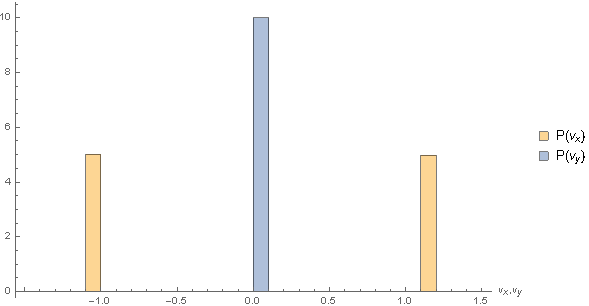
\includegraphics[clip=true,width=0.75\columnwidth]{histo_inicial.png}
    \caption{Distribución $P(v_x)$ y $P(v_y)$ a tiempo inicial.}
     \label{fig:histo_inicial}
\end{figure}

\ptitle{Condiciones de contorno}
Lo único que falta definir son las condiciones de borde, es decir, el mecanismo de interacción entre las partículas y la caja que las contiene. Para esto se consideró que cada pared actúa como un potencial repulsivo sobre cada partícula mediante la expresión
\[U^*(d_{ik}) = \frac{4}{d_{ik}^{12}},\]
donde $d_{ik}$ es la mínima distancia entre la partícula $i$ y la pared $k$ (se puede considerar $k = 1, 2, 3 \& 4$ representando las cuatro paredes de la caja). Este potencial se agrega en el cálculo de $F_i^{n}$ en la ecuación \ref{eq:Newton}. Una vez presentado queda claro por qué se eligió que ninguna partícula se encuentre en el borde de la caja a tiempo inicial: si esto ocurriera, $d_{ik} = 0$ para algún $k$ y, consecuentemente, $U(d_{ik})$ divergería produciendo una fuerza infinita sobre la partícula $i$, dando lugar a una situación inaceptable físicamente.

Se empleó el algoritmo de Verlet explicitado en las ecuaciones \ref{eq:Verlet} con $h = 0.005$ y un tiempo total de $20000$ pasos. Se verificó la conservación de la energía total del sistema calculada como $E_{tot} = E_{kin} + E_{pot}$ donde
\[E_{kin} = \sum_{i = 1}^{N^2} \frac{|v|^2}{2}\]
con $|v| = \sqrt{v_x^2 + v_y^2}$ y
\[E_{pot} = \sum_{i=1}^{N^2} \left( \sum_{j = 1, j \neq i}^{N^2} U(r_{ij})  + \sum_{k=1}^{4} U^*(d_{ik}) \right) \]
Además, se analizó la distribución de velocidades $P(v_x)$, $P(v_y)$, $P(v) = (P(v_x) + P(v_y))/2$ y $P(|v|)$.

\section{Resultados y discusión}

\ptitle{Conservación de la energía}

\begin{figure}[h]
    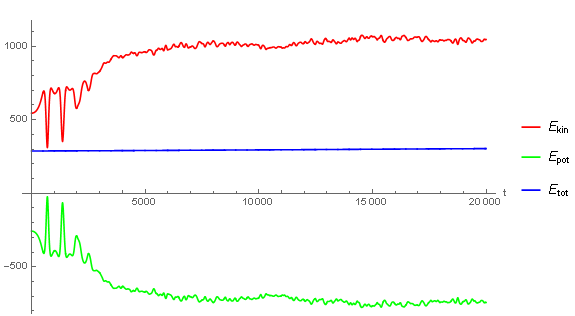
\includegraphics[clip=true,width=0.75\columnwidth]{energias.png}
    \caption{$E_{kin}$, $E_{pot}$ y $E_{tot}$ en función del tiempo.}
     \label{fig:energias}
\end{figure}

En primer lugar, se calculó $E_{kin}$, $E_{pot}$ y $E_{tot}$ para cada paso de tiempo y se observó que $E_{tot}$ se mantiene constante, tal como se verifica en la figura \ref{fig:energias}. Esto es consecuencia de que el sistema es conservativo y, además, el algoritmo de Verlet también lo es, respetando de este modo el comportamiento del sistema. Es importante aclarar que realmente esta cantidad se mantiene aproximadamente constante. Analizando por separado su comportamiento en la figura \ref{fig:energia_tot} y prestando especial atención a la escala en los ejes, se verifica que $E_{tot}$ aumenta en el tiempo. Esta desviación se atribuye a errores de redondeo, dado que disminuye a medida que $h$ se hace más pequeño. Debido a esto, se eligió un valor suficientemente pequeño para este parámetro con la condición de que el código ejecute en un tiempo razonable.

\begin{figure}[h]
    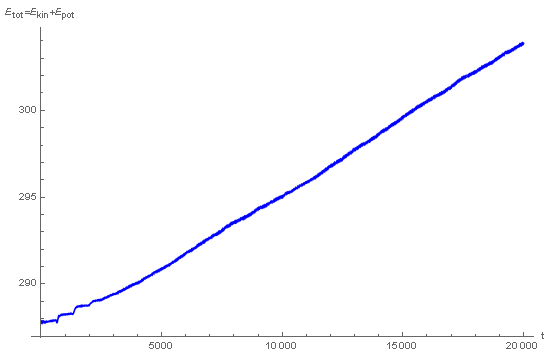
\includegraphics[clip=true,width=0.75\columnwidth]{energia_tot.png}
    \caption{$E_{tot}$ en función del tiempo. Nótese la diferencia de escala respecto a la figura \ref{fig:energia_tot}.}
     \label{fig:energia_tot}
\end{figure}


\ptitle{Distribuciones de velocidades}
En cuanto a los histogramas de velocidades a tiempo final graficados en la figura \ref{fig:histo_final}, se observan grandes diferencias respecto a aquellos a tiempo inicial (figura \ref{fig:histo_inicial}). En primer lugar, ambos se transformaron en distribuciones que asemejan a una distribución guassiana. En segundo lugar, arriban al mismo comportamiento a pesar de haber partido de condiciones iniciales distintas, lo cual implicaría que la forma de la distribución de velocidades a tiempo final es independiente de las condiciones iniciales. Esta afirmación se debería estudiar con más detalle.

\begin{figure}[h]
    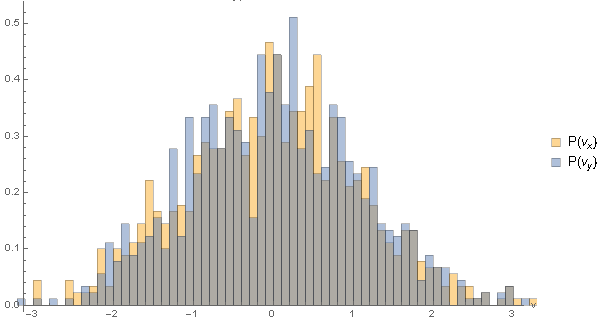
\includegraphics[clip=true,width=0.75\columnwidth]{histo_final.png}
    \caption{Distribuciones $P(v_x)$ y $P(v_y)$ a tiempo final.}
     \label{fig:histo_final}
\end{figure}

Además, en cuanto a $P(v)$ se obtuvo un comportamiento gaussiano igual a los anteriores, como se observa en la figura \ref{fig:histo_pv_final}. Esto es consecuencia directa de la definición de $P(v)$ como el promedio de las distribuciones $P(v_x)$ y $P(v_y)$.

\begin{figure}[h]
    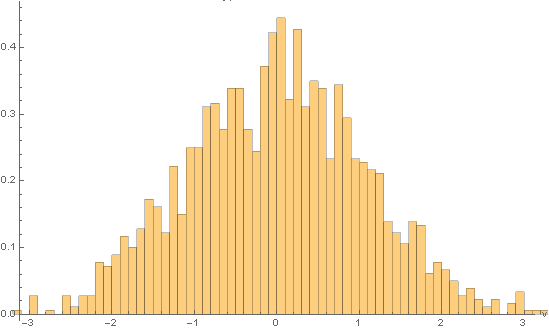
\includegraphics[clip=true,width=0.75\columnwidth]{histo_pv_final.png}
    \caption{Distribución $P(v)$ a tiempo final.}
     \label{fig:histo_pv_final}
\end{figure}


\ptitle{Distribución del módulo de la velocidad}

Por último, se analizó la distribución del módulo de las velocidades $P(|v|)$. Se obtuvo un comportamiento similar a la distribución de Maxwell-Boltzmann en dos dimensiones, tal como se observa en la figura \ref{fig:histo_pvmod_final}. Esta distribución de probabildiad es característica de la distribución de las velocidades de las moléculas en un gas ideal. Esto implica que el sistema modelado se comporta como un gas ideal, al menos en las condiciones utilizadas: $N = 900$, $L = 54.77$, densidad $\rho = N/L^2 = 0.3$.

\begin{figure}[h]
    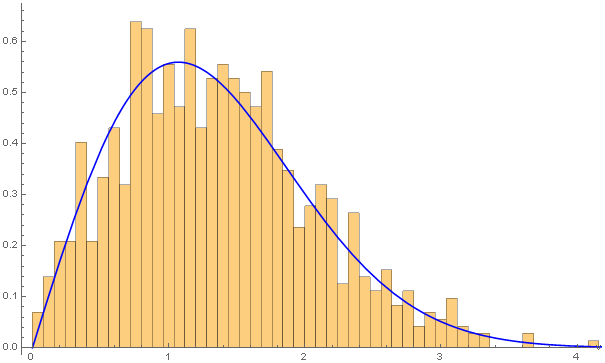
\includegraphics[clip=true,width=0.75\columnwidth]{histo_pvmod_final.png}
    \caption{Distribución $P(|v|)$ a tiempo final.}
     \label{fig:histo_pvmod_final}
\end{figure}



\bibliography{Radiacion_de_cuerpo_negro}



\end{document}

